% Figure: cross-domain ordering guarantee of shmem_put_signal.
% Referenced in main_spec.tex as fig:put-signal-xdomain.
% Regenerate PDF/PNG with:  make -C figures
\documentclass[border=3pt]{standalone}
% Shared preamble for the standalone figure sources in this directory.
% Fonts mirror ../utils/packages.tex so the generated figures match the
% specification's typography. tikz pulls in xcolor automatically.
\usepackage[T1]{fontenc}
\usepackage{mathptmx}
\usepackage[scaled=.90]{helvet}
\usepackage{courier}
\usepackage{tikz}
\usetikzlibrary{positioning,arrows.meta,fit,backgrounds,calc}

\begin{document}
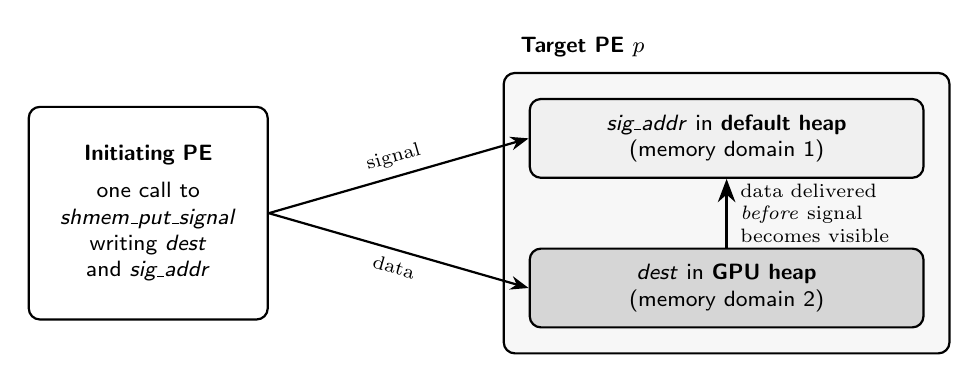
\begin{tikzpicture}[font=\footnotesize\sffamily, >=Stealth,
  dbox/.style={draw, thick, rounded corners, align=center,
               minimum width=5.0cm, minimum height=1.0cm}]
  \node[draw, thick, rounded corners, fill=white, align=center,
        text width=2.8cm, minimum height=2.7cm] (src)
        {\textbf{Initiating PE}\\[4pt] one call to\\ \textit{shmem\_put\_signal}\\ writing \textit{dest}\\ and \textit{sig\_addr}};
  \node[dbox, fill=black!6, right=3.3cm of src.east, yshift=0.95cm] (sig)
        {\textit{sig\_addr} in \textbf{default heap}\\(memory domain 1)};
  \node[dbox, fill=black!16, right=3.3cm of src.east, yshift=-0.95cm] (dest)
        {\textit{dest} in \textbf{GPU heap}\\(memory domain 2)};
  \begin{scope}[on background layer]
    \node[draw, thick, rounded corners, fill=black!3, inner sep=9pt, fit=(sig)(dest)] (pe) {};
  \end{scope}
  \node[font=\footnotesize\sffamily\bfseries, anchor=south west]
        at ([xshift=3pt, yshift=2pt]pe.north west) {Target PE $p$};

  \draw[->, thick] (src.east) to node[above, sloped, font=\scriptsize]{signal} (sig.west);
  \draw[->, thick] (src.east) to node[below, sloped, font=\scriptsize]{data}   (dest.west);
  \draw[->, very thick, black] (dest.north) -- (sig.south)
        node[midway, right=1pt, font=\scriptsize, align=left]
        {data delivered\\ \emph{before} signal\\ becomes visible};
\end{tikzpicture}
\end{document}
